% \setlength{\columnsep}{12pt}
% espaço entre colunas %\setlength{\columnseprule}{0.2pt} % linha vertical entre colunas

%-------------------------------------------------------------------------
% Modelo Trabalho PPGE-UFPB/Estatística
% Normas da ABNT
% Provedor: Laboratório de Economia e Modelagem Aplicada -- LEMA
%-------------------------------------------------------------------------

\documentclass[12pt, openright,oneside, a4paper, english, brazil]{report}

% ----------------------------
% Pacotes básicos 
% ----------------------------
% Fonte e codificação (acentuação)
\usepackage{lmodern}

\renewcommand{\sfdefault}{ppl}
\usepackage[T1]{fontenc}	
\usepackage[utf8]{inputenc}	
\usepackage[brazil]{babel}
\usepackage{comment} % para esconder a tabela Org do compilador
% Referências
%\usepackage[brazilian,hyperpageref]{}	
%\usepackage[alf]{abntex2cite}			
\usepackage[colon]{natbib}
\bibliographystyle{apalike}

%Texto aleatório
\usepackage{lipsum} 

% Tabelas e Figuras
\usepackage{ctable}             
\usepackage{multirow}
\usepackage{array}
\usepackage{float}              
\usepackage{longtable}          
\usepackage{xcolor,colortbl}    
\usepackage{booktabs}           
\usepackage{graphicx}			
\usepackage{subfig}             
\usepackage{caption}            
\usepackage{epstopdf}           

% Equações e símbolos
\usepackage{amsmath}            
\usepackage{nomencl} 
\usepackage{hyperref, cleveref}  

% Texto
\usepackage{indentfirst}		
\usepackage{color}				
\usepackage{microtype} 			
\usepackage{lastpage}			
% ----------------------------------------------------------
% Configurações do texto
% ----------------------------------------------------------
\usepackage{multicol}
\usepackage{array}
\newcolumntype{L}[1]{>{\raggedright\let\newline\\\arraybackslash\hspace{0pt}}m{#1}}
\newcolumntype{C}[1]{>{\centering\let\newline\\\arraybackslash\hspace{0pt}}m{#1}}
\newcolumntype{R}[1]{>{\raggedleft\let\newline\\\arraybackslash\hspace{0pt}}m{#1}}

\makeatletter
%\hypersetup{pdftitle={\@title}, pdfauthor={\@author}}
\makeatother

\def\preambulo{Trabalho elaborado em cumprimento às exigências da disciplina \disciplina, ministrada pela professor Dr. \professor.}
%--------------------------------------------------------------

\setlength{\parindent}{1.25cm}
\setlength{\parskip}{0.1cm} 

\usepackage{titlesec}
\usepackage{lipsum}

\makeindex




\title{Agenda 2030\\
{\normalsize Avaliação do avanço no Brasil dos Objetivos de Desenvolvimento Sustentável 01 Erradicação da pobreza e 02 Fome zero e agricultura sustentável da Agenda 2030}}
\def\autor{Jhonatan \\
Oscar Sérgio Monteiro\\
Vinícius Dutra}
\def\disciplina{SC329 - Sustentabilidade  Ambiental e Social, turma b}
\def\professor{Elcídio Henriques  Quiraque}
\begin{document}
\makeatletter
\begin{titlepage}
    \begin{figure}[H]
    \vspace{-3cm}
    \centering
    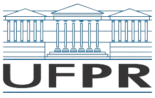
\includegraphics[height=3cm,keepaspectratio]{config/coverpage}\hfill
    \par\vspace{1cm}
    \end{figure}
    \begin{figure}[H]
    \vspace{-2cm}
    \centering
    
\includegraphics[height=3cm,keepaspectratio]{config/contabeis.png}
    \par\vspace{1cm}
    \end{figure}
     
    \vspace{2cm}
    
	\begin{center}
	    {\huge \bfseries \@title}
	    \begin{flushright}
		\begin{minipage}{8cm}
			\preambulo
		\end{minipage}
	\end{flushright}
	\vspace{3cm}
	    \normalsize
	    \autor
	\end{center}
	
\vfill
\centering
{\large Curitiba-PR, \the\year}

\end{titlepage}
\makeatother


\pdfbookmark[0]{\contentsname}{toc}
\tableofcontents
\newpage


\titleformat{\chapter}[display]{\normalfont\bfseries}{}{0pt}{\Huge  \thechapter. }
\newcommand{\doubletoprule}{%
  \specialrule{.1em}{2pt}{2pt}%
  \specialrule{.1em}{0pt}{0pt}%
}

\chapter{Introdução}
\section{Objetivos de Desenvolvimento Sustentável}
Os Objetivos de Desenvolvimento Sustentável são a evolução dos Objetivos de Desenvolvimento do Milênio, que foram propostos na Cúpula do Milênio em 2000, Nova York. Reunião promovida pela ONU que teve representantes de 189 países. Esse documento propôs o linhas de ação:
\begin{itemize}
\item redução da pobreza extrema,                                                  
\item educação,                                                                    
\item igualdade de gênero,                                                         
\item saúde,                                                                       
\item sustentabilidade ambiental,                                                  
\item combate a doenças,                                                           
\item parceria global para o desenvolvimento.
\end{itemize}
Os Objetivos de desenvolvimento foram revisados na Cúpula das Nações Unidas de 2015, Nova York. Essa reunião  observou que: a questão da sustentabilidade deveria ser melhor detalhada abordando questões de consumo e produção sustentável; a preocupação com as questões climáticas, que não foi um ODM, deveria receber destaque; a finitude e a dependência dos recursos hídricos deveria receber um destaque; o problema se sustentabilidade deve ser tratado de forma universal e não se restringe ao desafio nas nações em desenvolvimento.
\begin{quotation}   	     	"A nova Agenda se baseia nos Objetivos de Desenvolvimento do Milênio e pretende completar o que estes não alcançaram, particularmente em alcançar os mais vulneráveis. "
\end{quotation}
A cúpula de 2015 definiu os seguintes 17 Objetivos de Desenvolvimento Sustentável:
\begin{itemize}
\item  1 – Erradicação da pobreza    
\item  2 – Fome zero e agricultura sustentável                                 
\item  3 – Saúde e bem-estar                                                   
\item  4 – Educação de qualidade                                               
\item  5 – Igualdade de gênero                                                 
\item  6 – Água potável e saneamento                                           
\item  7 – Energia acessível e limpa                                           
\item  8 – Trabalho decente e crescimento econômico                            
\item  9 – Indústria, inovação e infraestrutura                                
\item  10 – Redução das desigualdades                                          
\item  11 – Cidades e comunidades sustentáveis                                 
\item  12 – Consumo e produção responsáveis                                    
\item  13 – Ação contra a mudança global do clima                              
\item  14 – Vida na água                                                       
\item  15 – Vida terrestre                                                     
\item  16 – Paz, justiça e instituições eficazes                               
\item  17 – Parcerias e meios de implementação Se quiser, posso também colocar
 \end{itemize}
 \chapter{Sobre a Agenda 2030}
 \section{Considerações sobre o documento}
O documento Agenda 2030, sem ser alarmista, chama a atenção para a necessidade premente de enfrentar os desafios que ameaça a humanidade:

\begin{quotation}
``Encontramo-nos num momento de enormes desafios para o desenvolvimento sustentável. Bilhões de cidadãos continuam a viver na pobreza e a eles é negada uma vida digna. Há crescentes desigualdades dentro dos e entre os países. Há enormes disparidades de oportunidades, riqueza e poder. A desigualdade de gênero continua a ser um desafio fundamental. O desemprego, particularmente entre os jovens, é uma grande preocupação. Ameaças globais de saúde, desastres naturais mais frequentes e intensos, conflitos em ascensão, o extremismo violento, o terrorismo e as crises humanitárias relacionadas e o deslocamento forçado de pessoas ameaçam reverter grande parte do progresso do desenvolvimento feito nas últimas décadas.''\\
...\\
``O esgotamento dos recursos naturais e os impactos negativos da degradação ambiental, incluindo a desertificação, secas, a degradação dos solos, a escassez de água doce e a perda de biodiversidade acrescentam e exacerbam a lista de desafios que a humanidade enfrenta. A mudança climática é um dos maiores desafios do nosso tempo e seus efeitos negativos minam a capacidade de todos os países de alcançar o desenvolvimento sustentável. Os aumentos na temperatura global, o aumento do nível do mar, a acidificação dos oceanos e outros impactos das mudanças climáticas estão afetando seriamente as zonas costeiras e os países costeiros de baixa altitude, incluindo muitos países menos desenvolvidos e os pequenos Estados insulares em desenvolvimento. A sobrevivência de muitas sociedades, bem como dos sistemas biológicos do planeta, está em risco.''\\
\end{quotation}
Notadamente o texto considera o caráter liberal das "Ralações Internacionais", enfatizando que os desafios podem e devem ser tratados pela cooperação e parceria.\\
Porem as reflexões sobre causas do não atingimento das metas das ODM não são apresentadas.\\
Ao reafirmar o reconhecimento da soberania dos estados ...\
\begin{quotation}
  "Reafirmamos que cada Estado tem, e exerce livremente, sua soberania plena e permanente sobre toda a sua riqueza, seus recursos naturais e sua atividade econômica. Vamos implementar a Agenda para o pleno benefício de todos, para a geração de hoje e para as gerações futuras. Ao fazê-lo, reafirmamos nosso compromisso com o direito internacional e enfatizamos que a Agenda deverá ser implementada de uma forma consistente com os direitos e obrigações dos Estados sob o direito internacional."
\end{quotation}
O Texto revela a fragilidade da proposta se vista a luz das correntes Realistas das relações dos Estados Nações. Essa corrente de pensamento trata como fundamentál a responsabilidade dos Estados Soberanos com a segurança e desenvolvimento  dos seus cidadãos, tendo os Governos restrição de legitimidade para abrir mão da sua soberania em prol da segurança e desenvolvimento de cidadãos de outros estados.\cite{jackson_sorensen_relacoes_internacionais} \\
\section{Metas definidas para a Erradicação da Pobreza.}
A Agende 2030 definiu as sequentes metas para a erradicação da pobreza:
\begin{itemize}
\item    1.1 até 2030, erradicar a pobreza extrema para todas as pessoas em todos os   lugares, atualmente medida como pessoas vivendo com menos de US\$ 1,25 por dia.
\item    1.2 até 2030, reduzir pelo menos à metade a proporção de homens, mulheres e crianças, de todas as idades, que vivem na pobreza, em todas as suas dimensões, de acordo com as definições nacionais. 
\item    1.3 implementar, em nível nacional, medidas e sistemas de proteção social apropriados, para todos, incluindo pisos, e até 2030 atingir a cobertura substancial dos pobres e vulneráveis.
\item    1.4 até 2030, garantir que todos os homens e mulheres, particularmente os pobres e vulneráveis, tenham direitos iguais aos recursos econômicos, bem como acesso a serviços básicos, propriedade e controle sobre a terra e outras formas de propriedade, herança, recursos naturais, novas tecnologias  apropriadas e serviços financeiros, incluindo microfinanças.
\item    1.5 até 2030, construir a resiliência dos pobres e daqueles em situação de vulnerabilidade, e reduzir a exposição e vulnerabilidade destes a eventos extremos relacionados com o clima e outros choques e desastres econômicos, sociais e ambientais.
\item    1.a garantir uma mobilização significativa de recursos a partir de uma variedade de fontes, inclusive por meio do reforço da cooperação para o desenvolvimento, de forma a proporcionar meios adequados e previsíveis para que os países em desenvolvimento, em particular os países de menor desenvolvimento relativo, implementem programas e políticas para acabar com a pobreza em todas as suas dimensões.
\item    1.b criar marcos políticos sólidos, em níveis nacional, regional e internacional, com base em estratégias de desenvolvimento a favor dos pobres e sensíveis a gênero, para apoiar investimentos acelerados nas ações de erradicação da pobreza. 
\end{itemize}
\section{Metas definidas para a acabar com a fome, alcançar a segurança alimentar e melhoria da nutrição e promover a agricultura sustentável}
\begin{itemize}
\item 2.1 Até 2030, acabar com a fome e garantir o acesso de todas as pessoas, em particular os pobres e pessoas em situações vulneráveis, incluindo crianças, a alimentos seguros, nutritivos e suficientes durante todo o ano 
\item 2.2 Até 2030, acabar com todas as formas de desnutrição, incluindo atingir, até 2025, as metas acordadas internacionalmente sobre nanismo e caquexia em crianças menores de cinco anos de idade, e atender às necessidades nutricionais dos adolescentes, mulheres grávidas e lactantes e pessoas idosas 
\item 2.3 Até 2030, dobrar a produtividade agrícola e a renda dos pequenos produtores de alimentos, particularmente das mulheres, povos indígenas, agricultores familiares, pastores e pescadores, inclusive por meio de acesso seguro e igual à terra, outros recursos produtivos e insumos, conhecimento, serviços financeiros, mercados e oportunidades de agregação de valor e de emprego não agrícola
\item  2.4 Até 2030, garantir sistemas sustentáveis de produção de alimentos e implementar práticas agrícolas resilientes, que aumentem a produtividade e a produção, que ajudem a manter os ecossistemas, que fortaleçam a capacidade de adaptação às mudanças climáticas, às condições meteorológicas extremas, secas, inundações e outros desastres, e que melhorem progressivamente a qualidade da terra e do solo
\item 2.5 Até 2020, manter a diversidade genética de sementes, plantas cultivadas, animais de criação e domesticados e suas respectivas espécies selvagens, inclusive por meio de bancos de sementes e plantas diversificados e bem geridos em nível nacional, regional e internacional, e garantir o acesso e a repartição justa e equitativa dos benefícios decorrentes da utilização dos recursos genéticos e conhecimentos tradicionais associados, como acordado internacionalmente 
\item 2.a Aumentar o investimento, inclusive via o reforço da cooperação internacional, em infraestrutura rural, pesquisa e extensão de serviços agrícolas, desenvolvimento de tecnologia, e os bancos de genes de plantas e animais, para aumentar a capacidade de produção agrícola nos países em desenvolvimento, em particular nos países menos desenvolvidos 
\item 2.b Corrigir e prevenir as restrições ao comércio e distorções nos mercados agrícolas mundiais, incluindo a eliminação paralela de todas as formas de subsídios à exportação e todas as medidas de exportação com efeito equivalente, de acordo com o mandato da Rodada de Desenvolvimento de Doha 
\item 2.c Adotar medidas para garantir o funcionamento adequado dos mercados de commodities de alimentos e seus derivados, e facilitar o acesso oportuno à informação de mercado, inclusive sobre as reservas de alimentos, a fim de ajudar a limitar a volatilidade extrema dos preços dos alimentos
\end{itemize}
\chapter{Agenda 2030 no Brasil}
\section{Ações no Governo Federal}
O Governo Federal criou a  Comissão Nacional para os Objetivos de Desenvolvimento Sustentável - CNODS, vinculada à Secretaria-Executiva da Secretaria-Geral da Presidência da República, com a participação de várias instituições como IPEA, IBGE, Fiocruz, Itaipu Binacional, Ministério do Planejamento e Orçamento e Ministério das Relações Exteriores.
O monitoramento é feito pelo  Relatório Nacional Voluntário, o ultimo publicado foi no ano de 2024.
O governo Federal se declara comprometido  com a ONU nos seus programas de sustentabilidade.
Segundo o governo federal a lei 14.802/2024 que é o PPA 2024 (Plano Plurianual 2024 - 2027) é um marco na retomada da capacidade de planejamento das ações publicas federais, este plano tem a Agenda 2030 como um importante referencial.
O RNV destaca ainda as ações de planejamento que corroboram com a Agenda 2030: Reformas estruturais e politica de inovação ; o Novo PAC (Programa de Aceleração do Crescimento); Nova Industria Brasil; Politica de Migração e Adaptação Climática; Programa de Aquisição de Alimentos; Ações de Defesa a Democracia; Programas de Incentivo a Cultura;Ações multidimensionais para a promoção do trabalho decente e dignidade;Programas de incentivo ao esporte e ; diversas comissões com o proposito de incentivar a participação social: Comissão Nacional de População e Desenvolvimento (CNPD), Conselho Nacional dos Direitos da Pessoa Idosa (CNDI), Conselho Nacional de Política Indigenista (CNPI), comitês voltados para os direitos de grupos LGBT-QIA+, crianças e adolescentes, bem como conselhos dedicados à ciência, tecnologia e inovação (CCT), segurança alimentar e nutricional (CONSEA, CAISAN) e meio ambiente (CONAMA, Comitê Interministerial de Mudança do Clima).
\begin{itemize}
\item ODS01: Erradicação da Pobreza
\begin{itemize}
\item Programa Bolsa Família (2003 / Reestruturado em 2023): Criado originalmente pela Lei nº 10.836/2003 e relançado com novas diretrizes pela Lei nº 14.601/2023.
\item Cadastro Único - CadÚnico (2001): Instituído pelo Decreto nº 3.877/2001 e consolidado pelo Decreto nº 6.135/2007 como o principal instrumento de seleção social do país.
\item Benefício de Prestação Continuada - BPC (1993): Criado pela LOAS em 1993 e regulamentado pelo Decreto nº 1.744/1996 (atualizado pelo Decreto nº 6.214/2007).
\item Lei Orgânica da Assistência Social — LOAS (Lei nº 8.742/1993): Regulamenta a assistência social e o Sistema Único de Assistência Social (SUAS).
\item Programa Minha Casa, Minha Vida (2009 / Retomado em 2023): Criado pela Lei nº 11.977/2009 e reformulado pela Lei nº 14.620/2023.
\end{itemize}
\item ODS 2: Fome Zero e Agricultura Sustentável
\begin{itemize}
\item Plano Brasil Sem Fome (2023): Lançado pelo Decreto nº 11.679/2023 com a meta de tirar o Brasil do Mapa da Fome até 2030.
\item Programa de Aquisição de Alimentos - PAA (2003 / Recriado em 2023): Instituído pela Lei nº 10.696/2003 e reestruturado pela Lei nº 14.628/2023.
\item Programa Nacional de Alimentação Escolar - PNAE (1955 / Marco Legal em 2009): Origem na década de 1950, com a obrigatoriedade da compra da agricultura familiar fixada pela Lei nº 11.947/2009.
\item Plano Safra da Agricultura Familiar / PRONAF (1995): O Programa Nacional de Fortalecimento da Agricultura Familiar foi criado em 1995 (Decreto nº 1.946/1996), com edições anuais do Plano Safra.
\item Lei Orgânica de Segurança Alimentar e Nutricional — LOSAN (Lei nº 11.346/2006): Cria o SISAN e estabelece o direito humano à alimentação adequada.
\item Lei da Agricultura Familiar (Lei nº 11.326/2006): Define as diretrizes e critérios de apoio aos pequenos produtores.
\item Lei de Combate ao Desperdício de Alimentos (Lei nº 14.016/2020): Regulamenta a doação de excedentes alimentares por estabelecimentos comerciais e feiras.
\item Política Nacional de Agroecologia e Produção Orgânica - PNAPO (2012): Instituída pelo Decreto nº 7.794/2012.
\item Garantia-Safra (2002): Criado pela Lei nº 10.420/2002 para mitigar perdas agrícolas decorrentes de secas ou enchentes.
\end{itemize}
\end{itemize}
\section{Considerações sobre o Relatório Nacional Voluntário de 2024}
Programas
segundo o RNV de 2024 para as 169 metas da Agenda a situação se resume:m
14 Atingidas
35 Sem evolução
26 Sem Evolução
23 Involução
71 Sem indicadores.
Em relação ao ODS 1 Erradicação da Pobreza o relatório declara:
\begin{quotation}
  "Houve poucos avanços na redução da pobreza extrema nos últimos dez anos.A pandemia teve um impacto negativo notável no ODS 1. Com uma breve que da pobreza extrema em 2020 por causa do Auxílio Emergencial, houve um aumento significativo em 2021, após a interrupção desse auxílio. A recuperação do mercado de trabalho e a retomada das transferências sociais contribuíram para uma nova queda em 2022. No entanto, para que as metas do ODS 1 sejam atingidas até 2023, o Brasil ainda precisa reduzir anualmente a taxa de pobreza extrema em cerca de 0,4 ponto percentual (p.p.). As disparidades na incidência da pobreza persistem entre diferentes regiões e grupos. As taxas mais altas estão nas regiões norte e nordeste, entre a população preta e parda e nas áreas rurais. A redução da pobreza multidimensional tem sido mais positiva do que a redução da pobreza monetária, embora haja desafios na obtenção de dados regulares para monitoramento. Programas de transferência de renda, como o Bolsa Família, desempenham um papel crucial na redução da pobreza. A nova fase do Bolsa Família, iniciada em 2023, amplia a cobertura e os valores transferidos, com foco na proteção à primeira infância, representando uma iniciativa inspiradora para outros países em desenvolvimento na luta contra a pobreza.  Em relação a Erradicar a Fome O Brasil enfrenta desafios significativos em relação ao ODS 2. Embora a fome seja uma questão antiga no país, o conceito de Segurança Alimentar e Nutricional surgiu nos anos 1980. Desde então, foram desenvolvidas políticas e programas para combater a fome e promover a segurança alimentar ao mesmo tempo, como o Programa Fome Zero, lançado em 2003. Com isso, entre 2004 e 2013, houve progresso significativo na redução da fome e o Brasil, em 2014, saiu do Mapa da Fome da Organização das Nações Unidas (ONU) pela primeira vez. No entanto, os anos seguintes foram marcados por uma crise econômica e política, que resultou no aumento da insegurança alimentar, agravado pela pandemia. Os dados mais recentes mostram que 9,4\% dos domicílios do Brasil estavam em insegurança alimentar moderada ou grave em 2023, indicando uma redução de 3,3 p.p. em relação a 2017-2018, mas 1,6 p.p. acima de 2013. Portanto, é necessário ainda um esforço conjunto do governo, da sociedade civil e do setor privado para promover políticas e programas que garantam o acesso a alimentos nutritivos e suficientes para toda a população, especialmente a mais vulnerável. Por essa razão, o PPA 2024-2027 enfatiza o enfrentamento da insegurança alimentar e da pobreza como prioridades, além do fortalecimento da agricultura familiar e do agronegócio sustentável.
\end{quotation}
\href{https://odsbrasil.gov.br/objetivo1/indicador111}{Indicadores da CNODS} 
\section{Governo do Estado do Paraná}
\begin{itemize}
\item ODS 1: Erradicação da Pobreza
\begin{itemize}
\item Programa Cartão Comida Boa (2020 / Tornado Permanente em 2021): Criado emergencialmente pelo Decreto nº 4.570/2020 e transformado em programa estruturante contínuo pela Lei Estadual nº 20.747/2021.
\item Fundo Estadual de Combate à Pobreza — FECOP (Lei Estadual nº 18.573/2015): Destina recursos orçamentários específicos para a redução das desigualdades.
\item Agências do Trabalhador (Rede SINE - 1975 / Expansão PR nos Anos 1990): Intermediação pública de empregos integrada ao Sistema Nacional de Emprego.
\item Plano Estadual de Habitação de Interesse Social - PEHIS-PR (2010): Diretrizes plurianuais para urbanização e moradia popular no estado.
\end{itemize}
\item ODS 2: Fome Zero e Agricultura Sustentável
\begin{itemize}
\item Programa Compra Direta Paraná (2020): Instituído pela Lei Estadual nº 20.252/2020 para compra direta de alimentos de cooperativas familiares.
\item IDR-Paraná - Instituto de Desenvolvimento Rural (2019): Criado pela Lei Estadual nº 20.121/2019 com a fusão de órgãos estaduais (Emater, Iapar, CPRA e Clap).
\item Banco de Alimentos Comida Boa / CEASA-PR (2020): Programa de arrecadação, triagem e reaproveitamento de alimentos reestruturado no âmbito das Centrais de Abastecimento do PR.
\item Programa Cozinha Escola (2021): Iniciativa de capacitação profissional em gastronomia sustentável e reaproveitamento de alimentos.
\item Lei Estadual de SAN (Lei nº 16.292/2009) e CONSEA-PR: Criação do SISAN estadual e fortalecimento do Conselho Estadual de SAN.
\item Lei Estadual da Agroecologia (Lei nº 16.739/2010): Estabelece o incentivo à produção agrícola orgânica no estado.
\item Plano Estadual de Segurança Alimentar e Nutricional - PESAN-PR (2012 / Atualizações Periódicas): Instrumento de planejamento governamental para erradicação da fome.
\end{itemize}
\end{itemize}
\section{Prefeitura de Curitiba (Âmbito Municipal)}
\begin{itemize}
\item  ODS 1: Erradicação da Pobreza
\begin{itemize}
\item Fundação de Ação Social - FAS (1993): Criada pela Lei Municipal nº 8.353/1993 para coordenar a assistência social na cidade.
\item Plano Municipal de Assistência Social - PMAS (Elaboração Quadrienal): Documento normativo que estabelece as diretrizes dos CRAS e CREAS locais.
\item Liceu de Ofícios (1993) e Espaço Empreendedor (2013): Programas municipais focados na capacitação profissional, formalização de pequenos negócios e geração de renda.
\item Programa Câmbio Verde (1989): Projeto pioneiro de troca de recicláveis por hortifrúti frescos da agricultura familiar.
\end{itemize}
\item ODS 2: Fome Zero e Agricultura Sustentável
\begin{itemize}
\item Programa Mesa Solidária (2019): Instituído para oferecer gratuitamente refeições diárias com dignidade à população vulnerável em espaços próprios.
\item Armazéns da Família (1989) e Sacolões da Família (1996): Rede pública de abastecimento com preços subsidiados mantida pelo município.
\item Restaurantes Populares de Curitiba (2007): Inauguração da primeira unidade (Matriz) em 2007, expandindo-se pelas regionais da cidade.
\item Programa de Hortas Comunitárias (1986) e Fazenda Urbana do Cajuru (2020): Estímulo à agricultura urbana local; a primeira Fazenda Urbana foi inaugurada em 2020.
\item Lei da Agricultura Urbana (Lei Municipal nº 15.300/2018): Marco legal que disciplina o uso sustentável de áreas urbanas para cultivo de alimentos.
\item Secretaria Municipal de Segurança Alimentar e Nutricional - SMSAN (2017): Criada pela Lei Municipal nº 15.004/2017 para gerir a política de abastecimento social.
\item COMSEA Curitiba (2003): Conselho Municipal instituído pela Lei nº 10.741/2003 para garantir a participação popular nas políticas alimentares.
\end{itemize}
\end{itemize}

Programa Alimenta Curitiba (2018): Estratégia municipal voltada à promoção da educação alimentar e combate ao desperdício nas redes pública  s de ensino e abastecimento.

\section{Ações da Sociedade Civil}
Na sociedade civil existe o "Grupo de Trabalho da Sociedade Civil para a Agenda 2030 de Desenvolvimento Sustentável"  formada por 50 entidade.\\
\href{https://gtagenda2030.org.br/quem-faz/}{lista de instituições GT Agenda 2030}\\
Este grupo publica anualmente um relatório de acompanhamento dos indicadores no Brasil.\\
\href{https://gtagenda2030.org.br/quem-faz/agenda2030.org.br/wp-content/uploads/2025/09/relatorio-luz-2025.pdf}{Relatório Luz 2025}

Pela analise do ``Relatório Luz 2025'' as Metas 1.1,1.2,1.3 as ações foram consideradas satisfatórias, em relação as metas 1.4,1.5,1.a houve retrocesso, para a meta 1.b o relatório indica estagnação.

Para as metas do ODS 2 o Relatório classifica as ações para as metas 2.1,2.3 como satisfatórias , para as metas 2.2,2.5,2.a insuficientes. Para a meta 2.b as acoes foram consideradas estagnada e as metas 2.4 e 2.c foram consideradas ameaçadas.

\chapter{Propostas concretas}

1. Hubs de Co-propriedade Comunitária (ODS 1)

Criação de cooperativas e microindústrias em áreas vulneráveis, nas quais os beneficiários do CadÚnico atuam como sócios e co-proprietários, combinando essa estrutura com creches estendidas e mobilidade local.

Ataca a raiz da pobreza ao trocar a dependência contínua de auxílios por geração e acúmulo de patrimônio real para as famílias.

2. Cinturões Alimentares de Compra Garantida (ODS 2)

Contratos governamentais e corporativos de longo prazo (5 a 10 anos) com agricultores familiares, oferecendo preço mínimo justo, apoio na transição agroecológica e seguro climático.

Elimina a ação de atravessadores e a especulação de preços, fixando o produtor no campo com estabilidade financeira e garantindo alimentos saudáveis e sem veneno para a cidade.

3. Upcycling Obrigatório e Economia Circular (ODS 2 + ODS 1)

Legislação que proíbe o descarte de resíduos orgânicos reaproveitáveis por indústrias e varejistas, exigindo a transformação industrial de subprodutos em novos alimentos (Upcycled Food) e a compostagem comunitária do restante.

Zera o desperdício na fonte ao redesenhar a cadeia de produção, criando empregos verdes locais e gerando biofertilizantes gratuitos para a agricultura urbana.


\chapter{Como as empresas podem incluir está ODS em seus planos de negócios}

1. Além do Salário Digno: Segurança de Vida e Emancipação do Trabalhador (ODS 1)
A raiz da pobreza urbana não é apenas a falta de renda, mas a pobreza de tempo, de saúde e de estabilidade. A empresa atua na raiz quando remove os custos invisíveis e o estresse estrutural que impedem o trabalhador de prosperar.

Soberania de Tempo e Infraestrutura de Vida:

Combate à Pobreza de Tempo: Implementação de semanas de trabalho reduzidas (ex: 32h ou 36h semanais) sem redução salarial para cargos operacionais/de menor renda, devolvendo tempo para estudo, convivência familiar e descanso.

Garantia de Moradia e Mobilidade: Criar auxílios de moradia atrelados à proximidade do trabalho (reduzindo o tempo de deslocamento em transporte público, que em grandes metrópoles consome até 4h/dia do trabalhador) ou parcerias para habitabilidade digna e acessível.

Distribuição de Riqueza e Co-propriedade (ESOPs / Participação Real):

Em vez de apenas pagar salários, criar programas de democratização do capital (Employee Stock Ownership Plans), onde funcionários operacionais se tornam acionistas e coproprietários da empresa, acumulando patrimônio real ao longo dos anos.

Formação e Emancipação Contínua:

Financiamento integral de educação formal (ensino técnico, graduação, idiomas) dentro da jornada de trabalho, garantindo que o colaborador tenha uma rota clara de ascensão profissional e autonomia financeira definitiva.

2. Cadeia de Suprimentos Responsável e Compras Regenerativas (ODS 2)
A raiz do problema na agricultura familiar é a vulnerabilidade do mercado e a margem de lucro esmagada pelos intermediários.

Contratos de Longo Prazo e Garantia de Preço Justo:

Estabelecer contratos plurianuais com pequenos produtores e cooperativas locais com garantia de compra e preço mínimo estipulado (Fair Trade de fato), eliminando a figura do atravessador.

Financiamento Antecipado da Transição Agroecológica:

A empresa assume o risco financeiro da transição do produtor (do cultivo tradicional/químico para o agroecológico), adiantando capital sem juros para insumos, certificações e infraestrutura sustentável no campo.

3. Redesenho Circular do Modelo de Negócios: Perda Zero na Fonte (ODS 2)
A gestão tradicional de resíduos trata o lixo no fim do processo (end-of-pipe). A abordagem radical redesenha a operação para que o desperdício seja estruturalmente impossível.

Industrialização e Upcycling Interno de Alimentos (Upcycled Food):

Em vez de "doar o que sobrou", a empresa altera seu processo produtivo para que subprodutos alimentares (cascas, talos, grãos processados) sejam transformados na própria fábrica em novos produtos de valor comercial ou nutricional.

Operação de "Loop Fechado" (Closed-Loop):

Integração total com a cadeia local: os resíduos orgânicos inevitáveis da empresa não vão para aterros; retornam diretamente aos agricultores parceiros na forma de compostagem corporativa e biofertilizantes, fechando o ciclo de nutrientes do solo.

4. Investimento Transformador e Construção de Riqueza Comunitária (ODS 1 e ODS 2)
A filantropia tradicional (doar cestas básicas) perpetua a dependência. O investimento radical gera autonomia econômica e infraestrutura comunitária.

Desenvolvimento de Negócios Sociais Locais (Community Wealth Building):

Em vez de doar recursos para ONGs assistenciais, a empresa investe fundo de capital (Venture Philanthropy) para fundar e incubar cooperativas e cozinhas comunitárias geridas pelos próprios moradores da comunidade do entorno.

Transferência de Tecnologia e Compras Locais Obrigatórias:

A empresa capacita e transfere tecnologia/máquinas para esses empreendimentos locais e se compromete, por estatuto, a comprar prioritariamente os produtos e serviços desenvolvidos por essas cooperativas da comunidade.
\bibliographystyle{apalike}
\bibliography{referencias}                                                     
 
\end{document}
